\chapter{Machine Learning Model Development}
\label{chap: model}

This chapter introduces an ML model development procedure used in both classification tasks in Chapter \ref{chap: rul} and regression tasks in Chapter \ref{chap: reg}. The procedure involves:
\begin{enumerate*}[label=(\alph*)]
    \item signal pre-processing,
    \item feature generation,
    \item feature selection,
    \item model training,
    \item model validation, and
    \item hyperparameter tuning,
\end{enumerate*}
as shown in Figure \ref{fig: model development}.

\begin{figure}[tb]
    \centering
    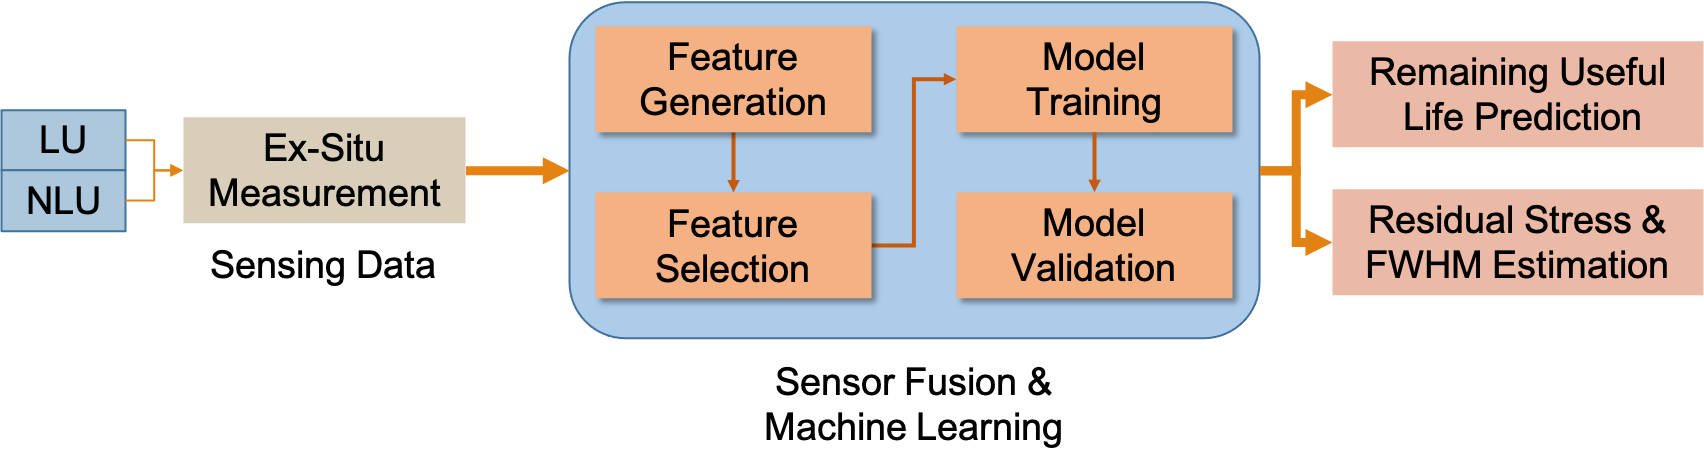
\includegraphics[width=\linewidth]{fig/model_development.png}
    \caption{Overview of the ML model development}
    \label{fig: model development}
\end{figure}

\section{Signal pre-processing}
It is essential to reduce noises and extract regions of interest in signals by signal processing before we perform analyses.x First, DC bias is removed by subtracting the mean amplitude from a signal to prevent models from fitting on the bias. Second, considering the computational cost from the high-resolution data, we choose to downsample the ultrasonic signals. Third, we define the region of interest as the interval containing the response of an ultrasonic signal, and thus the other parts of a signal are discarded so that redundant information is not included.

\section{Feature generation}
Since ultrasonic sensor signals are unstructured, which is difficult to be manipulated in an ML context, feature extraction methods are needed to create a representative set of values, i.e., features that aggregate the information from an entire signal. In this stage, physics-based and data-driven features are generated. The hybrid feature pool enables us to incorporate both physics knowledge and data-driven information into models.

\subsection{Physics-based features}
Given that physics modeling is built on theories or comprehensive experiment studies, physics-based features are robust, explainable, and suitable for applications having limited amounts of data such as the fatigue testing data in this research. Therefore, parameters (features) from traditional LU and NLU testings become potential candidates in the feature pool.
\begin{itemize}
    \item Wave velocity
    
    In LU testing, ultrasonic wave velocity is a stiffness-based measure that is associated with macroscopic damage such as crack/void coalescence and propagation. The wave speed is the distance divided by the time-of-flight that an ultrasonic wave propagating in a material, as shown by Equation \eqref{eq: wave velocity}
    
    \begin{equation}
        v = \frac{2D}{\Delta t}
        \label{eq: wave velocity}
    \end{equation}
    where wave velocity is denoted by $v$, and $D$ is the thickness of a specimen. $\Delta t$ is the time difference between the actuation pulse and the response signal. Notice that, in our LU testing setup, one transducer severs as both a transmitter and a receiver. Thus, the excitation signal travels $2D$ and the phase is changed $180^{\circ} $ when received, as illustrated in Figure \ref{fig: wave speed}.

    \begin{figure}[tb]
        \centering
        \begin{subfigure}[t]{0.49\linewidth}
            \centering
            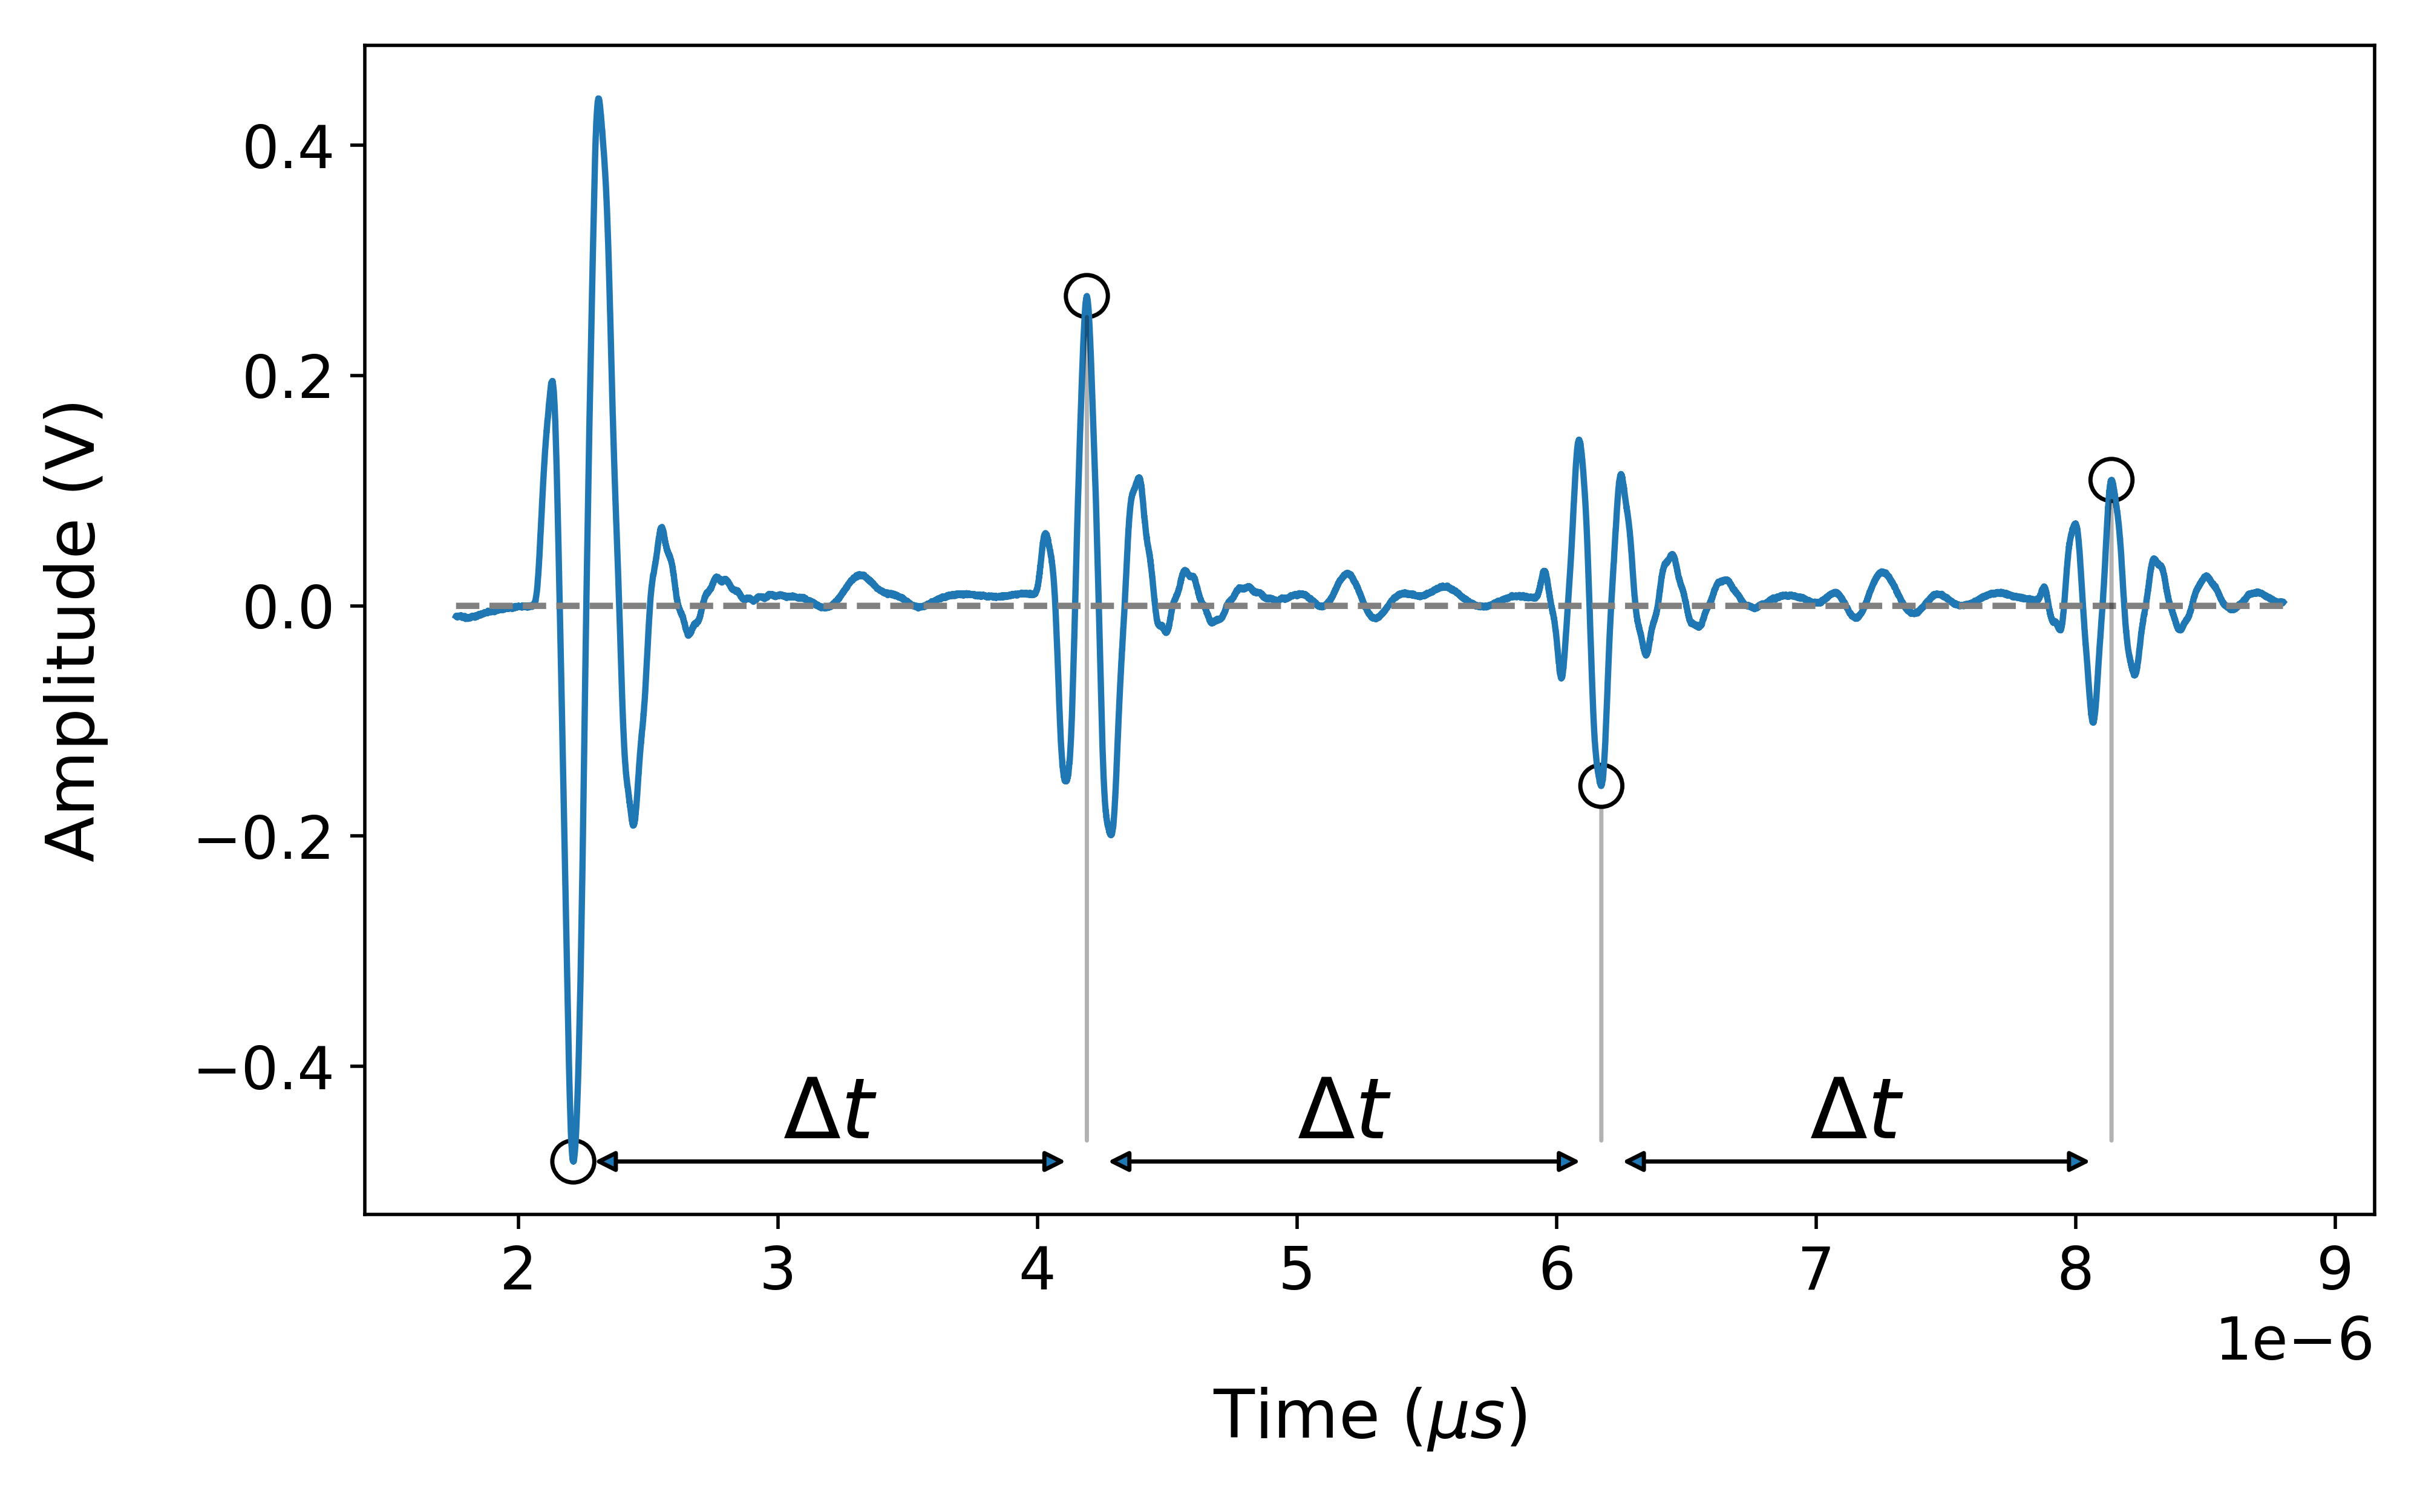
\includegraphics[width=\linewidth]{fig/wave_speed.png}
            \caption{Wave speeds from an LU signal}
            \label{fig: wave speed}
        \end{subfigure}
        \begin{subfigure}[t]{0.49\linewidth}
            \centering
            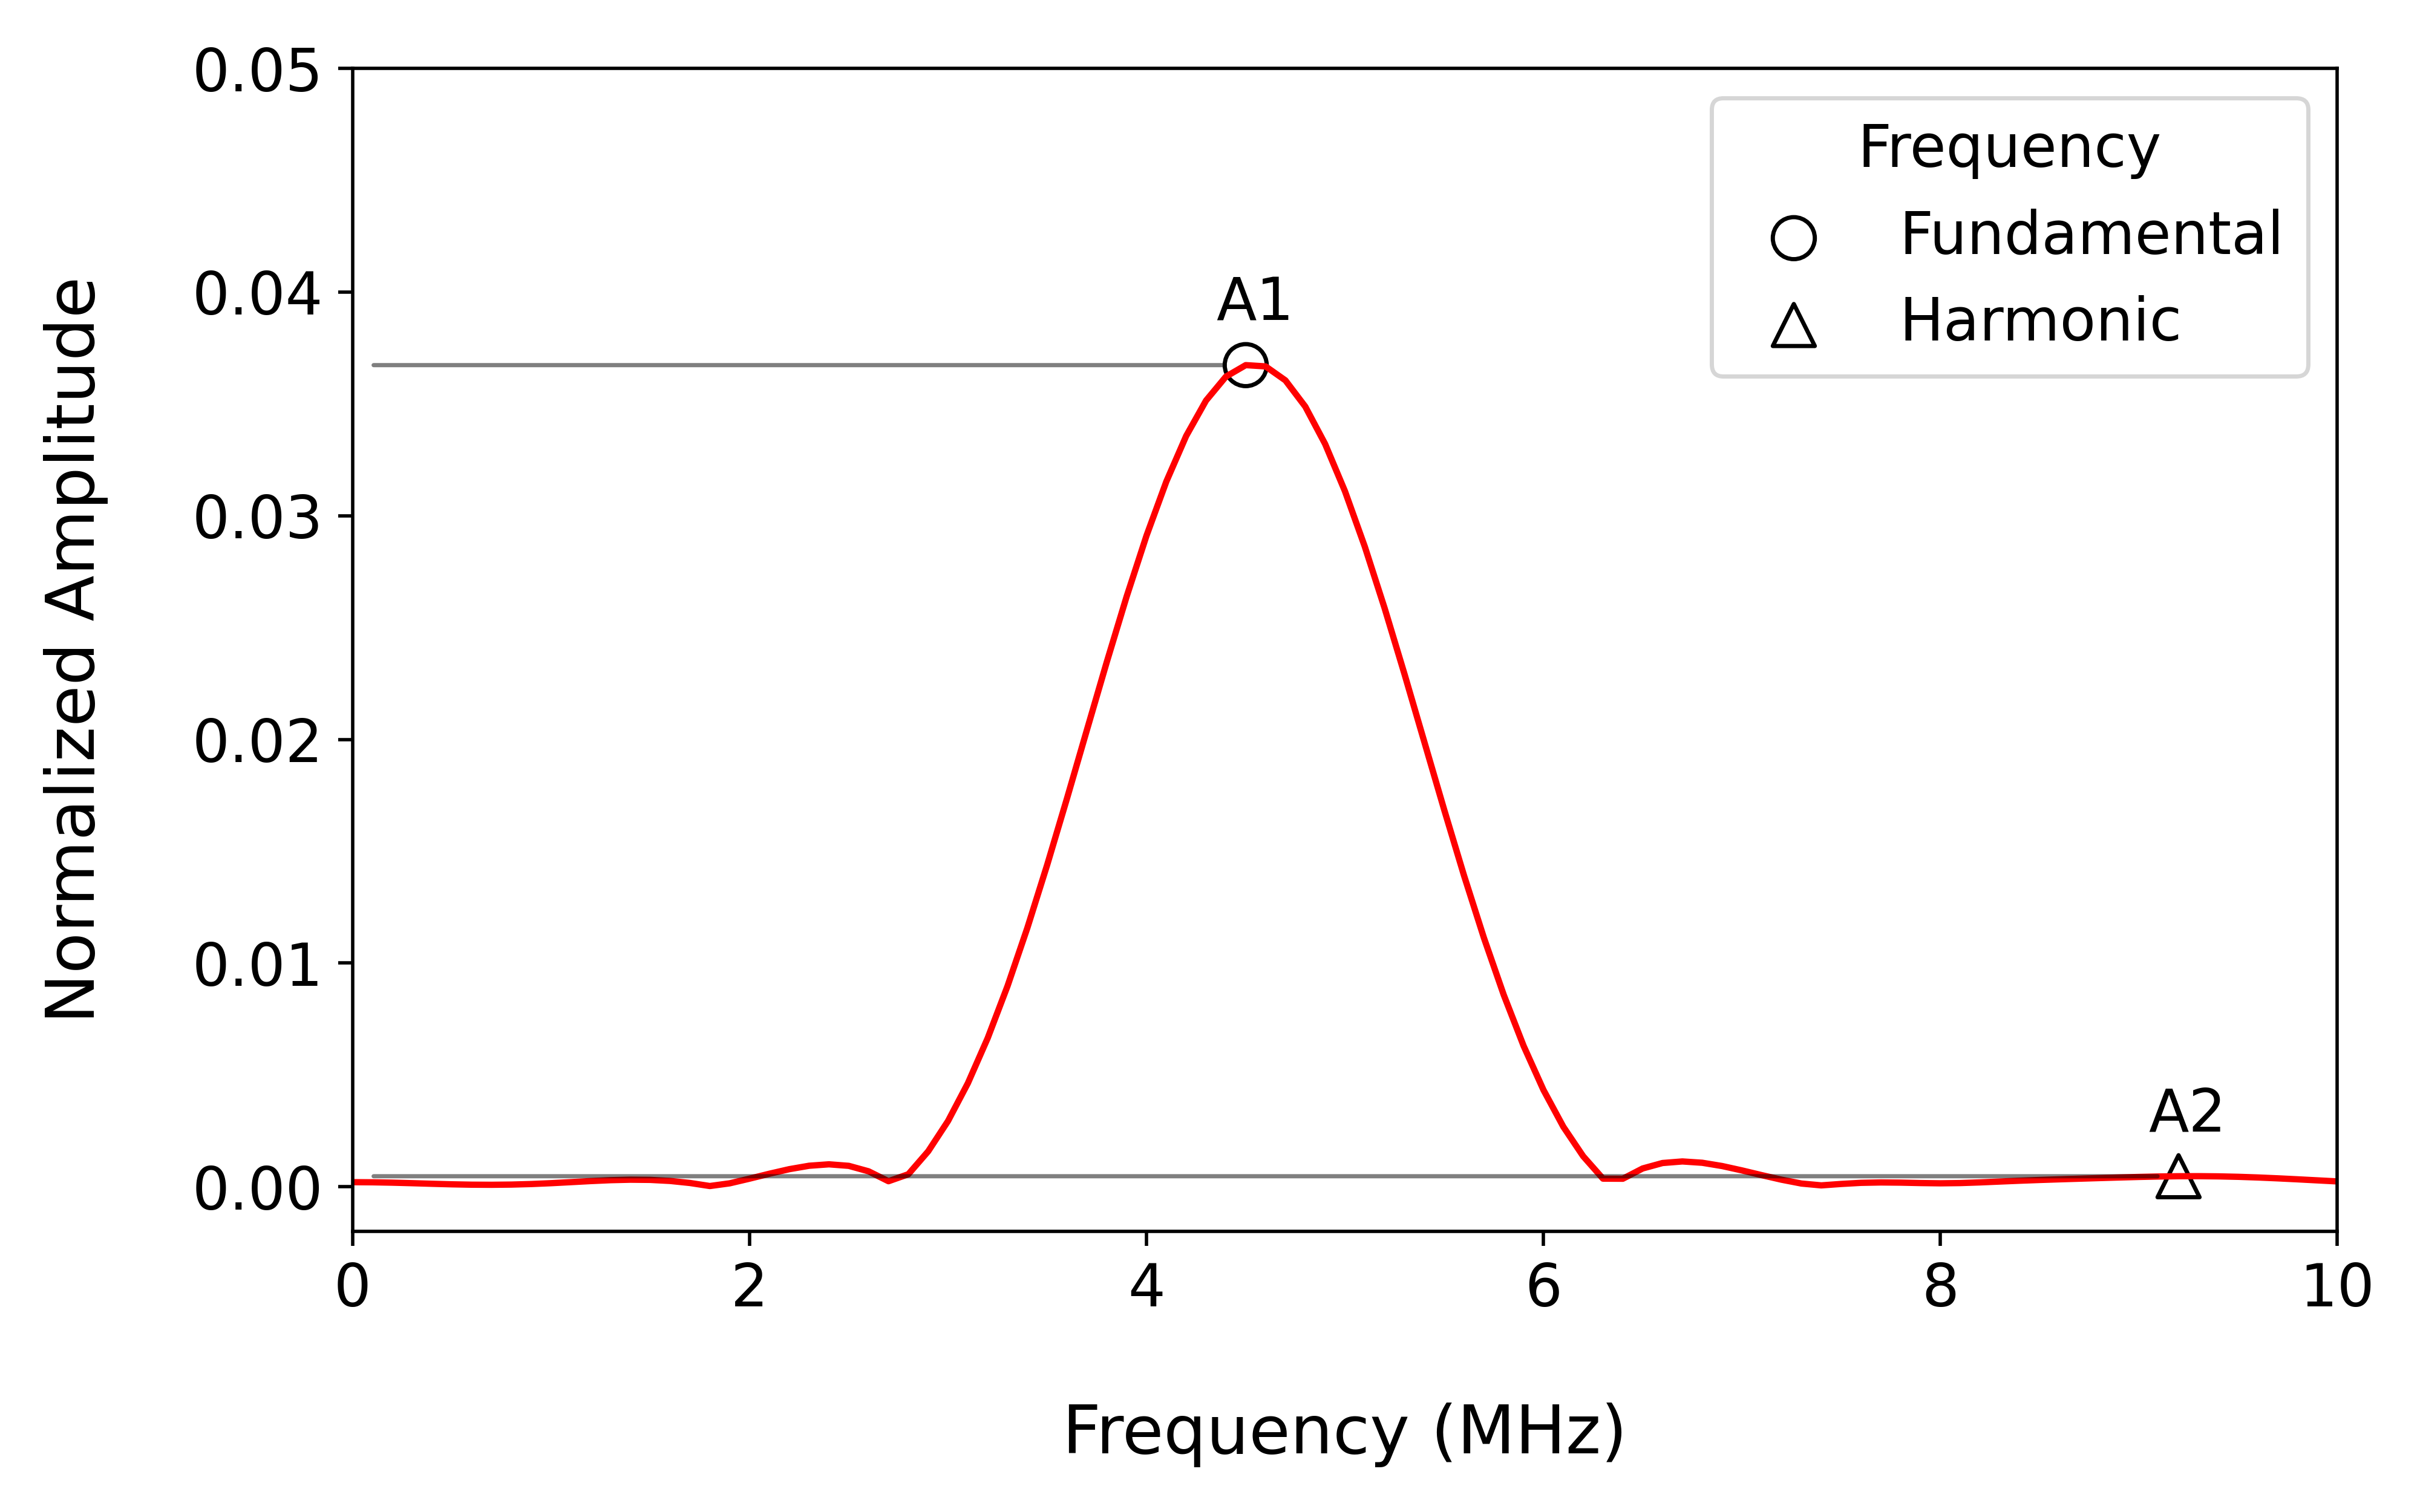
\includegraphics[width=\linewidth]{fig/beta.png}
            \caption{Nonlinear acoustic parameter from an NLU signal after FFT}
            \label{fig: beta}
        \end{subfigure}

        \caption{Calculation of physics-based features}
    \end{figure}

    

    \item Nonlinear acoustic parameter $\beta$
    
    While wave velocity from LU testing is able to detect fatigue damage at the macroscale, it is limited because it cannot detect defects much smaller than the probing wavelength, e.g., 1 mm. In contrast, NLU techniques are based on a different physical principle: nonlinear elasticity from nano- and micro-scale defects induce harmonic generation. The nonlinear acoustic parameter is related to the amplitude of generated harmonics \cite{nde-nlu-review-Matlack2014,nde-nlu-fatigue-Cantrell}. This nonlinear parameter changes due to defects such as dislocations, local plastic strain, precipitates, and micro-cracks, all of which are orders of magnitude smaller than the probing wavelength. Here, we apply fast Fourier transform (FFT) to NLU measurements and calculate the nonlinear parameter by using the ratio between the FFT amplitudes of the fundamental and the harmonic waves in Equation \eqref{eq: beta}

    \begin{equation}
        \beta = \frac{A_2}{A_1^2}
        \label{eq: beta}
    \end{equation}
    where $A_1$, $A_2$ is the FFT amplitude of the fundamental wave and the second-order harmonic wave, respectively. Figure \ref{fig: beta} displays the the fundamental and harmonic frequency and their amplitude in the frequency domain.
\end{itemize}

\subsection{Data-driven features}
The physics-based features alone, however, are not enough to capture all of the information from the LU and NLU signals. As a result, a large number of features engineered from the time domain, frequency domain, and time-frequency domain of ultrasonic measurements are added to the feature pool \cite{nde-lu-ml-defect-Sambath2011, nde-lu-ml-defect-s19194216}.

\begin{itemize}
    \item Time domain features
    
    The time domain features are peak amplitudes, ratios between peak amplitudes, and components from principal component analysis (PCA) and independent component analysis (ICA). Statistics in the time domain such as median, quantiles, variance, skewness, and kurtosis are also included. Besides, wave duration, wave energy, and the ratios between these quantities are calculated from the envelope analysis of an NLU signal.

    \item Frequency domain features
    
    Frequency domain analysis offers information that is not presented in the time domain. This information is especially valuable for periodic signals such as ultrasonic measurements. Thus, after applying FFT, peak amplitudes, ratios between peak amplitudes, peak frequencies, frequency centroid, and frequency variance in FFT spectrum are extracted as the frequency domain features.

    \item Time-frequency domain features
    
    Ultrasonic signals are usually not stationary, i.e., frequency changes in time, because of the interaction between ultrasonic waves and discontinuities within the material. Therefore, time-frequency analysis is needed to describe the phenomena. Discrete wavelet transform (DWT) is adopted to decompose ultrasonic measurements into several frequency bands, as an example in Figure \ref{fig: dwt decomposition}. Then, statistics such as mean, median, kurtosis, and skewness are recorded for each frequency band.
\end{itemize}

\begin{figure}[tb]
    \centering
    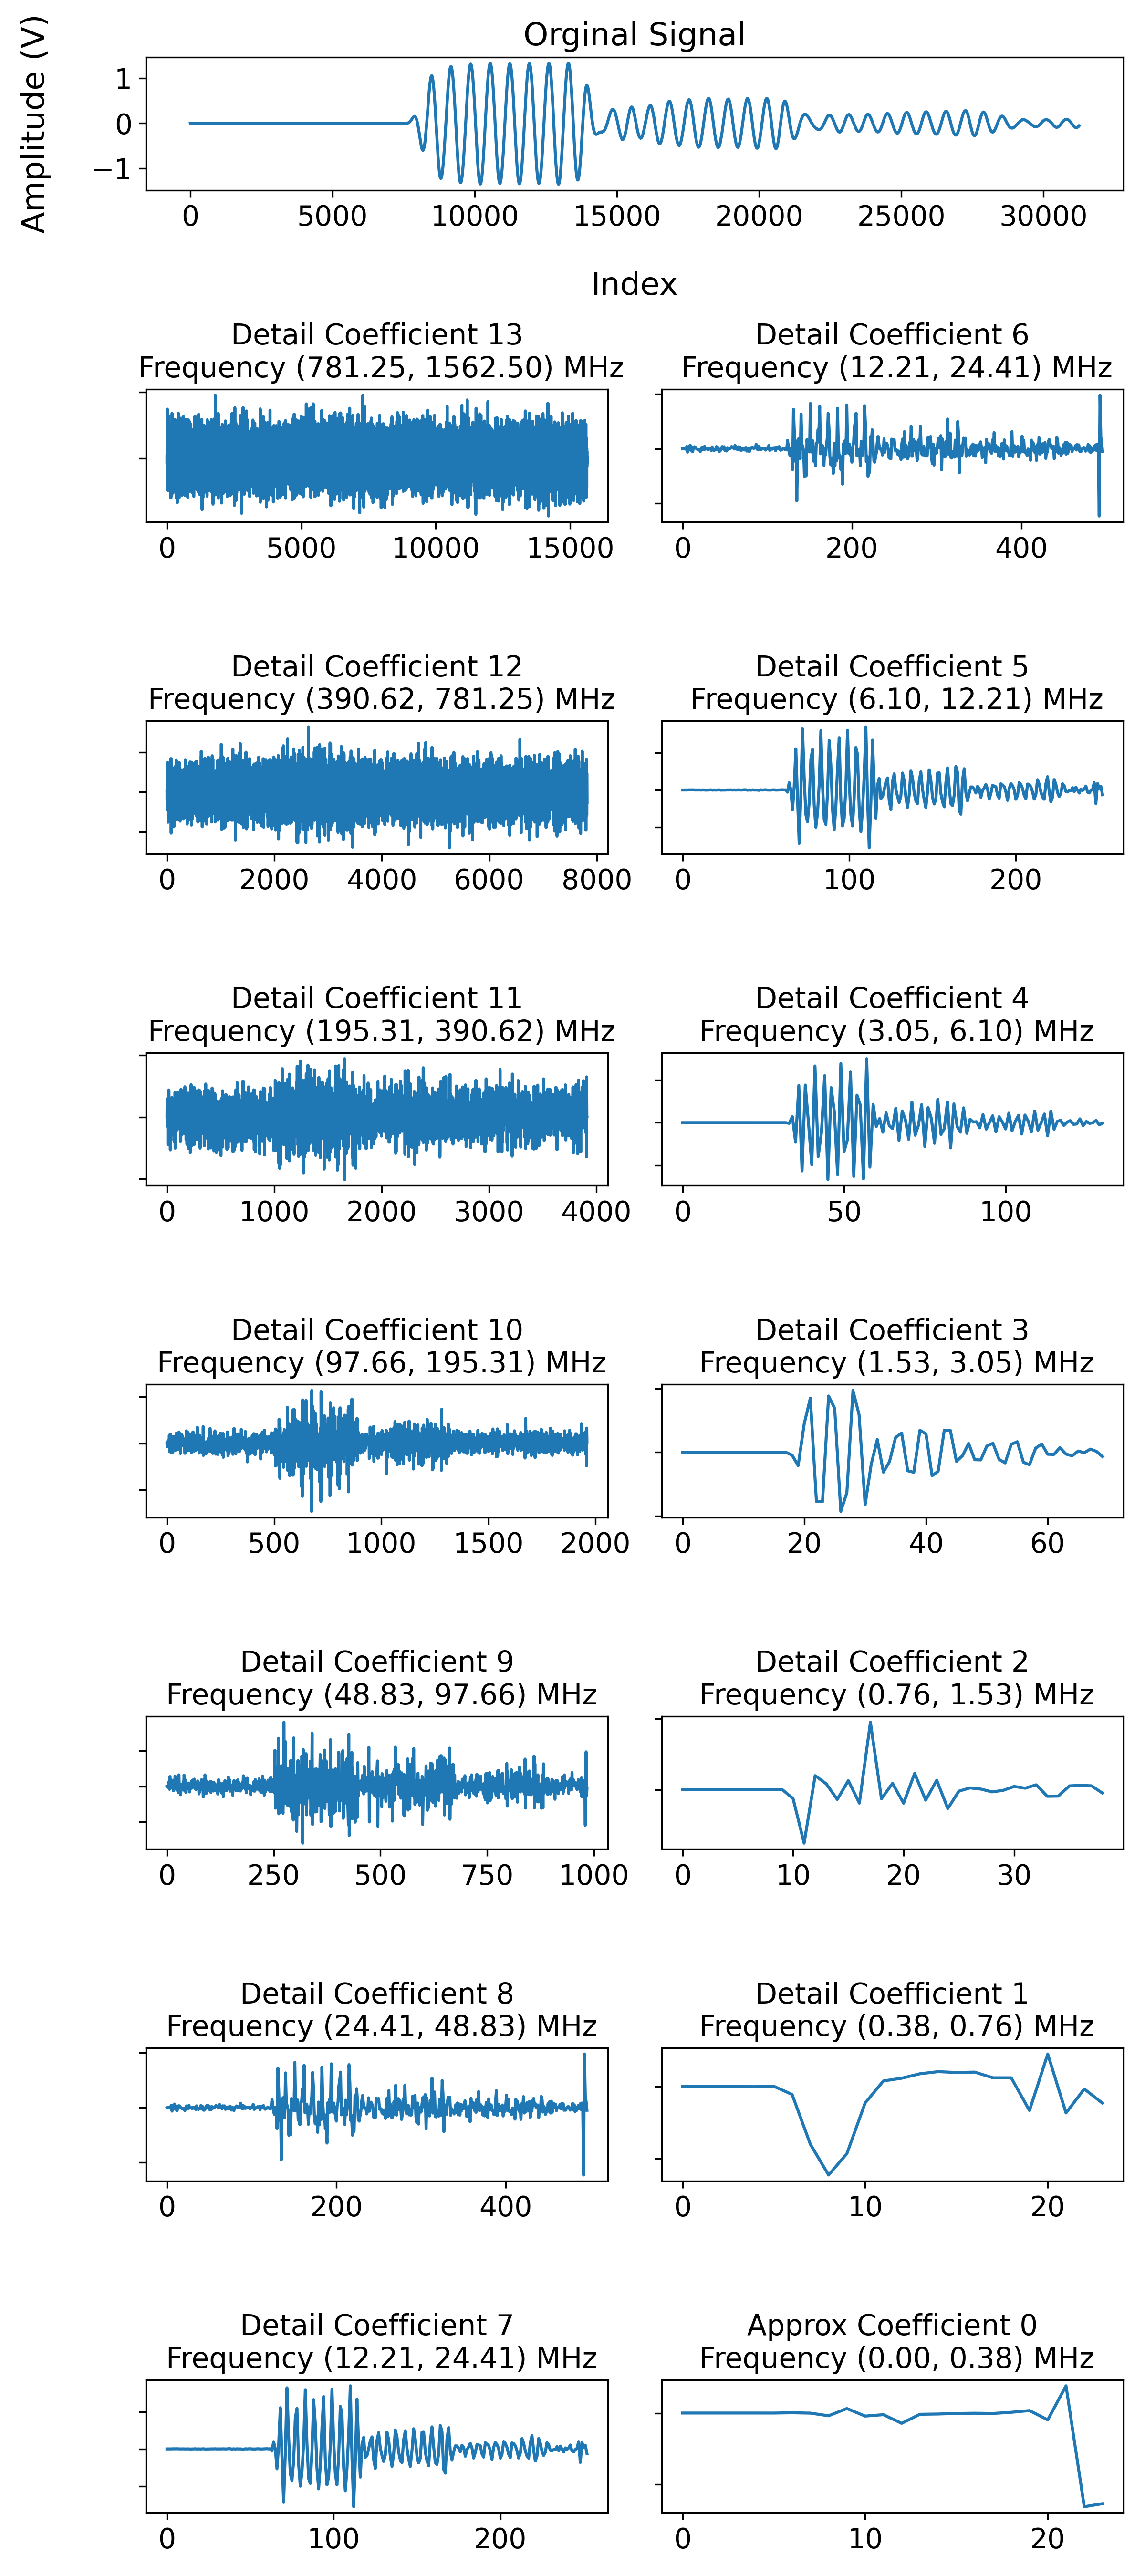
\includegraphics[height=\linewidth]{fig/dwt_decomposition.png}
    \caption{DWT decomposition of an NLU signal}
    \label{fig: dwt decomposition}
\end{figure}

We concatenate features from LU and NLU signals together, and the feature pool contains 191 features in total. Lists of candidate features for LU and NLU signal profiles are displayed in Appendix \ref{app: feature}.

\section{Feature selection}
Feature selection aims to remove redundant features. Irrelevant features are common to see when we construct features without fully understanding a physical process such as the relationship between fatigue mechanism and ultrasonic responses. By including only the best subset of features for a prediction task, feature selection is beneficial for developing robust models against overfitting and improving model generalizability. There exist various feature selection techniques which can be mainly classified into three categories: filter methods, wrapper methods, and embedded methods \cite{Guyon2002}. Each of these methods has its advantages, disadvantages, and applicable scenarios.

In the model development pipeline, we adopted a wrapper method, recursive feature elimination \cite{feature-selection-GUYON2003} with cross-validation (RFECV) to obtain an optimal feature subset that achieves the best predictive performance in multiple training/test data splits for a single model. The RFECV algorithm is depicted in Figure \ref{fig: rfecv}. First, recursive feature elimination (RFE) starts from a set with all available features and eliminates $k$ features step by step based on the feature ranking with regressors or classifiers until the predetermined number of features $n$ is reached. Nevertheless, the best number of features to select $n^*$ needs to be determined prior to the modeling. To find out $n^*$ while alleviating the problem of overfitting, cross-validation (CV) \cite{cv-kohavi1995study}, a statistical model validation technique, is used along with RFE. CV partitions a dataset into a training set and a validation set in each iteration. A model is evaluated multiple times with different partitions, and $n^*$ is determined by the overall validation results. Then, RFE selects the optimal $n^*$ features from the feature pool. We choose a 5-fold CV in this feature selection procedure to avoid adding too much computational cost due to the fact that RFE is already computationally expensive.

\begin{figure}[tb]
    \centering
    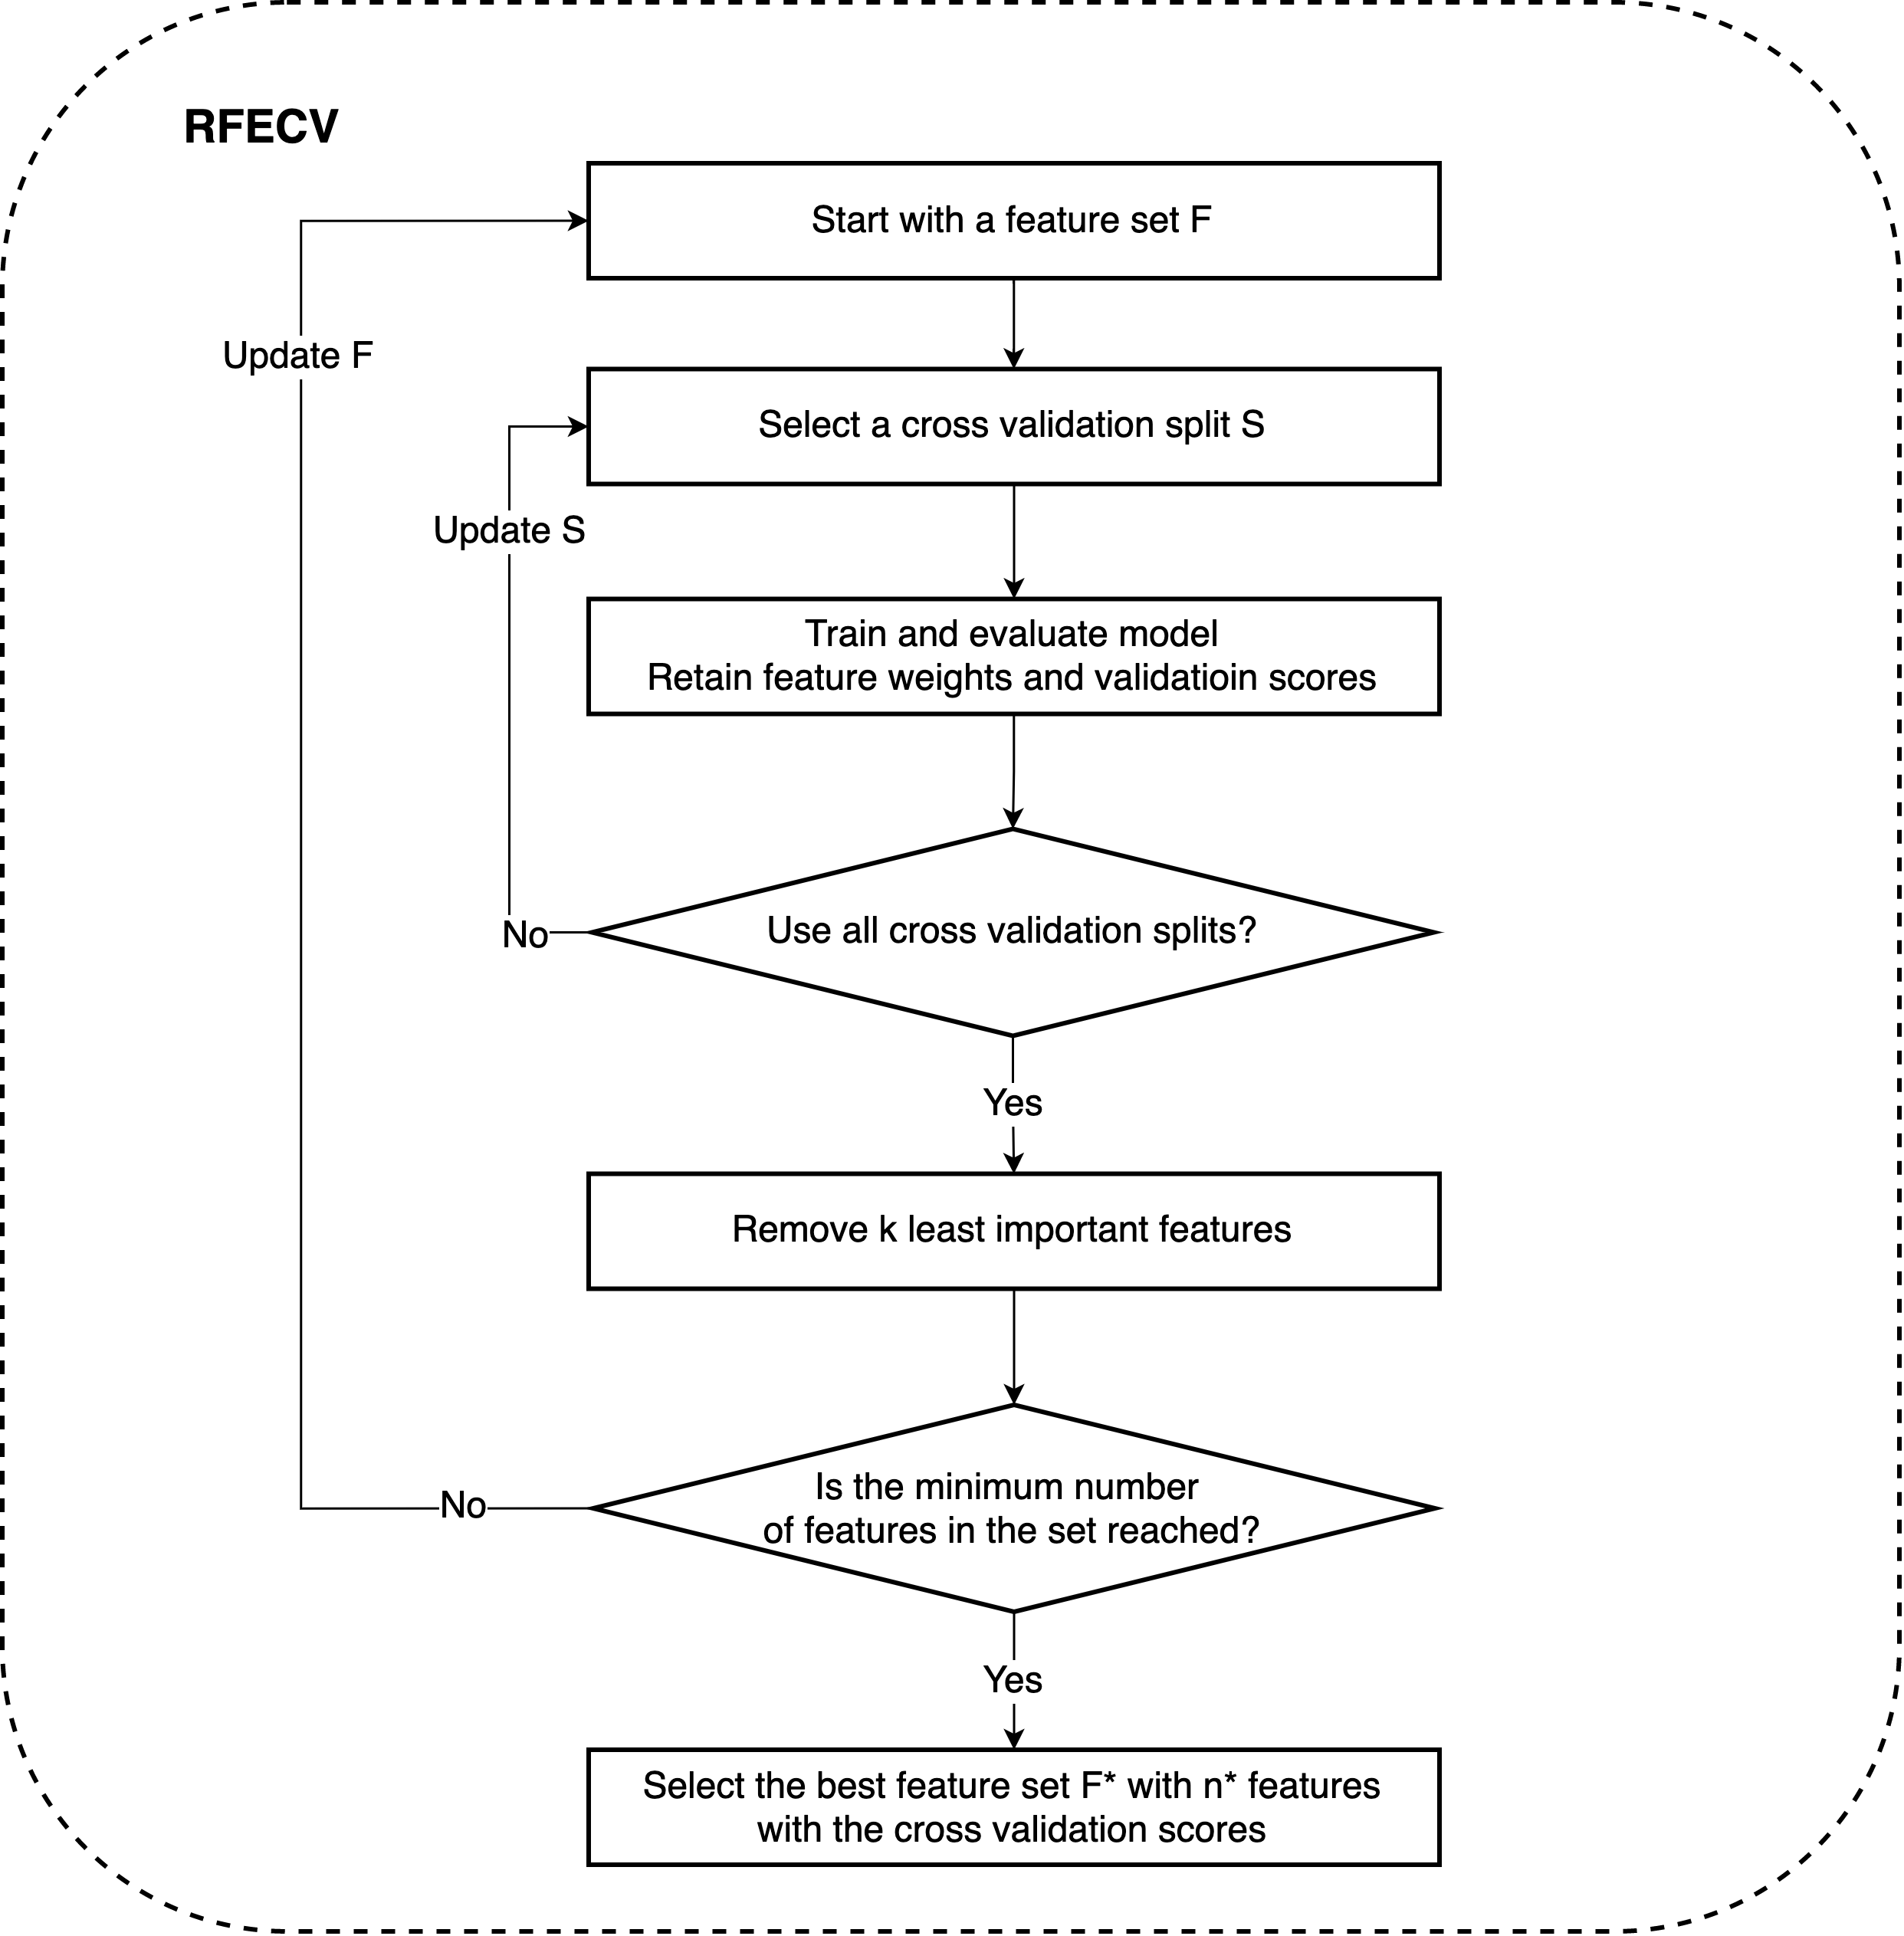
\includegraphics[width=0.9\linewidth]{fig/rfecv.png}
    \caption{Flowchart for feature selection with RFECV}
    \label{fig: rfecv}
\end{figure}

\section{Model training and validation}
\label{sec: model train and val}
Model training and validation involve another CV loop in Figure \ref{fig: logocv}. However, this CV is not for finding the best feature subset but for providing a generalized estimate of a model's performance. Specifically, leave-one-group-out CV (LOGOCV) \cite{LOGOCV-Saeb059774} is applied, where each group contains three repeated measurements at one measurement location on one specimen. Here, we make an assumption that each group, i.e., each measurement location on a specimen, is an independent sample because of the differences in the microstructure. In LOGOCV, each group is tested once and obtained validation scores by a predictor trained on the other groups, which efficiently utilizes the dataset and assesses the generalization capacity of a model.

\begin{figure}[tb]
    \centering
    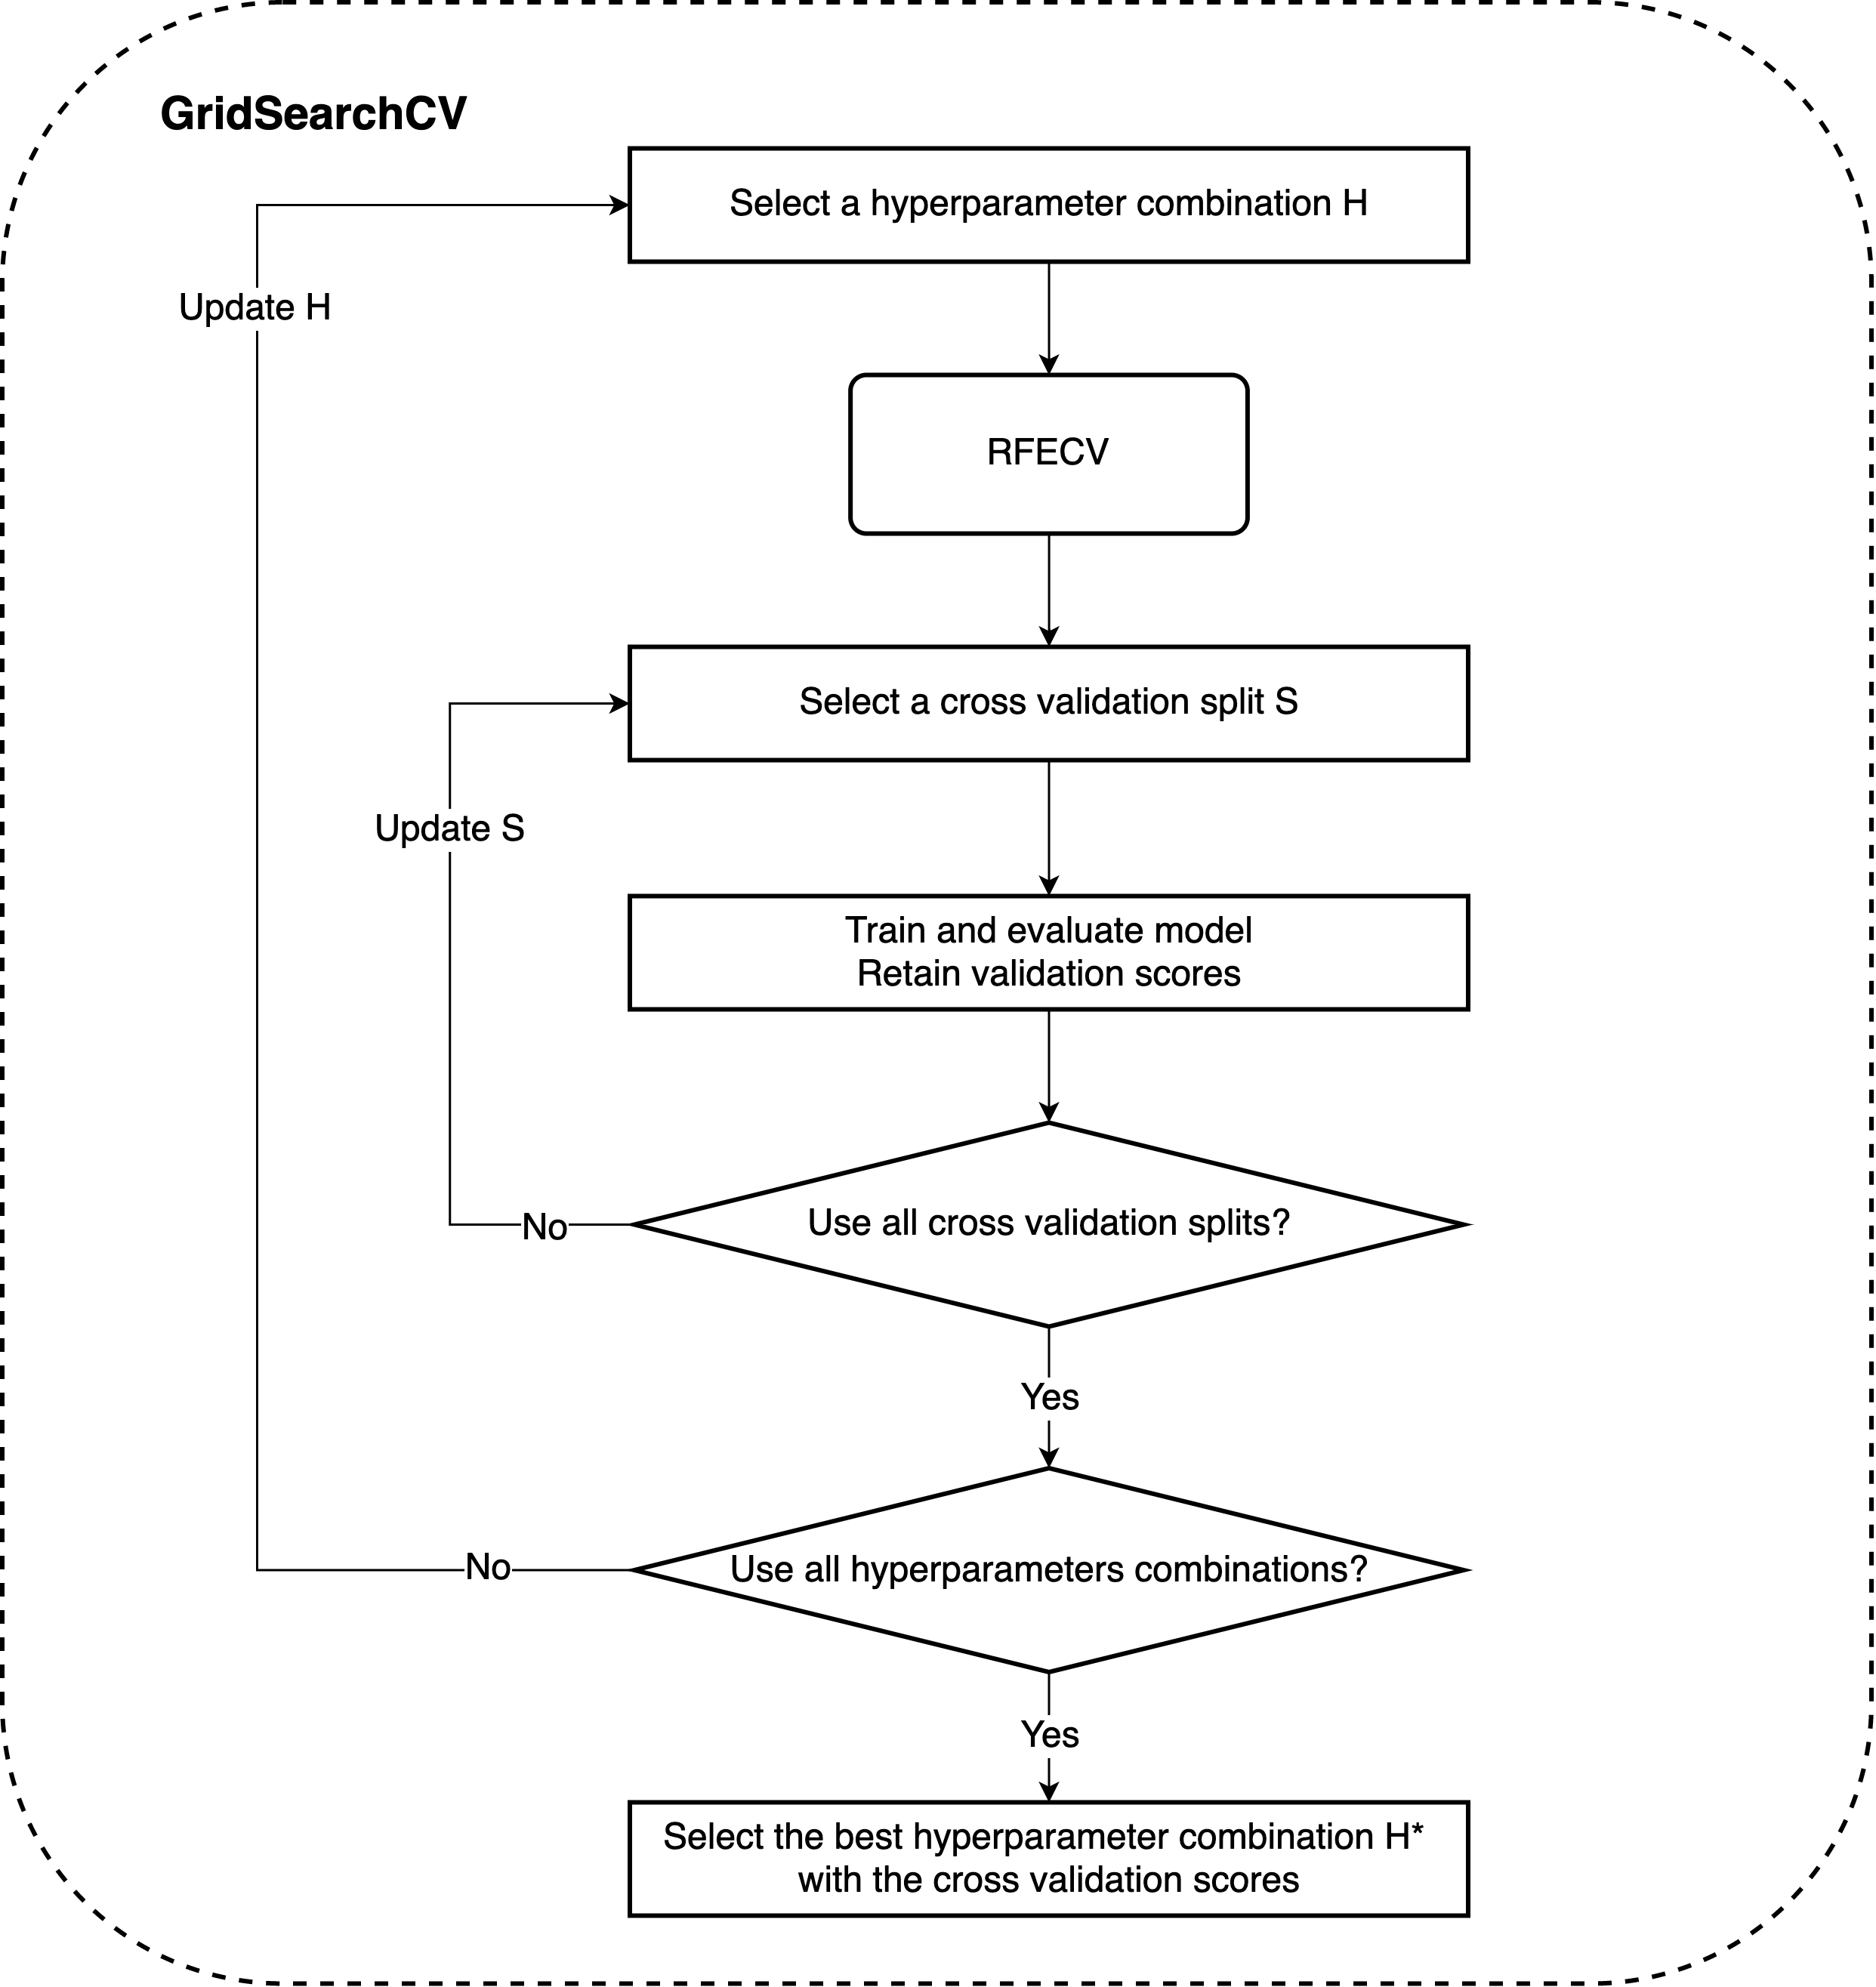
\includegraphics[width=0.9\linewidth]{fig/logocv.png}
    \caption{Flowchart for model training, validation, and hyperparameter tuning with grid search and LOGOCV}
    \label{fig: logocv}
\end{figure}

\section{Hyperparameter tuning}
Searching for an optimal set of hyperparameters is another critical step that significantly influences ML model performance. We use grid search \cite{hyperparameter-Feurer2019} accompanied with the validation scores from the LOGOCV result to tune hyperparameters in a simple manner, as depicted in Figure \ref{fig: logocv}. Grid search exhaustively considers all candidates from predefined hyperparameter combinations. Each combination is used to train a model, and the best hyperparameter set is the one achieving the best CV result. 

The number of hyperparameters and the range of each hyperparameter vary in different learning algorithms. The candidate algorithms includes: logistic regression, support vector machine (SVM), and random forest for classification in Chapter \ref{chap: rul}; linear regression, Lasso regression, SVM, and random forest for regression in Chapter \ref{chap: reg}.